\section{ENGINEERING REQUIREMENTS}

%\begin{slshape} 
%\color{blue}
%	This section constitutes the meat of the document. Remember that it is ''requirements" and not methods. The 
%	definition here should leave no doubt about what is needed.  Engineering requirements differ from stakeholder requirements in measurability, detail, and unambiguity.
%	\bigskip
%	
%	Measurability is a key attribute; without it we have no way of knowing that we have built what we said that we would build.  In the aerospace industry 
%	the process of determining that what we have built meets the plan to which we were building is called verification.  Verification answers the question,
%	``Did we build what we said we would build?"
%	\bigskip
%	
%	Ideally, detail in engineering requirements means that the designer can set off designing and building the system with little or no extra input from the stakeholders.  
%	Since we do not live in an ideal world additional stakeholder input will be required.  When additional input is sought the specification should be revised to reflect clarification
%	or change.  Reality is why we include a Revision History Block at the beginning of the specification.
%	\bigskip
%	
%	An ambiguous requirement, by its very nature, means that I could design and build the system in one, two, or many `wrong' ways.  Since the stakeholder who is paying for this system doesn't want one of the many possible wrong ways we need to ensure that requirements cannot be misinterpreted by the designer. 
% \bigskip
%	
%	
%	
%	Understand:
%		\begin{enumerate}
%			\item ``An engineering requirement is a statement about the system that is unambiguous. There's only one way it can be interpreted, 
%							and the idea is expressed clearly so all of the stakeholders understand it."
%			\item ``An engineering requirement is binding. The customer is willing to pay for it, and will not accept the system without it."
%			\item	``An engineering requirement is testable. It's possible to show that the system either does or does not comply with the statement." (Steve Tockey)
%		\end{enumerate}
%		
%Additionally, requirements must be stated in one place only in this document.  You can reference the requirement in another part of the document by using its paragraph number.  It is often tempting to restate a requirement in another requirement to improve clarity.  However, a requirement stated in two places may only get changed in one place during a revision and possibly  leading to confusion or worse a flawed product.
%\bigskip
%		
%Engineering requirements constitute contacts between between clients and design teams.  Requirements are binding.
%\bigskip		
%		
%Requirements form the base that we design on.  A well written requirement keeps us from ending up with a less than ideal implementation.  
%Defining requirements forces us to think prior to design.
%\bigskip
%		
%The engineer's job at this point is to make the stakeholder requirements of the previous section into measurable, detailed, and unambiguous.  
%Sometimes this process requires that a stakeholder be interviewed again until a proper set of engineering requirements emerge.
%\bigskip 
%
%An old joke in aerospace says that a specification is written and thrown over a high wall to the design group.  The spec. writer then runs away from the wall (laughing).  While formal adoption of this absurd method leads to disaster, we should write specifications as if we could never clarify anything.  The clearer we make the specification now, the lower the cost of change later.
%\bigskip
%
%
%
%\subsection*{\underline{Processing Stakeholder Requirements into Engineering Requirements}}
%
%Stakeholder requirements in the form of user stories are typically poorly organized and indefinite.  A designer cannot design to an indefinite requirement.  How would a designer know if an indefinite requirement was met?  Also, different stakeholders may have requirements that effect overlapping areas of the system but because of the nature of story collection the overlap in these requirements may not be obvious.  There are many more issues and a systematic approach to this processing problem should help. 
%\bigskip
%
%The work of sorting and firming up requirements can be considered tedious.  Engineers are famous for hating tedious work.  It is why we are constantly automating things that we don't want to do.  And when we encounter a tedious task we have a tendency to create a process to limit the amount of tedium that we must endure.  Tedious work reduced to a process becomes less tedious if the process is well designed.  In order to translate the scattered and indefinite stakeholder requirement into organized and definite engineering requirements we are going to follow a two step process:
%
%\begin{enumerate}
%\item Identify and sort stakeholder requirements into fixed categories.
%\item Rewrite the sorted requirements into definitive engineering requirements.
%\end{enumerate}
%
%The details of the process are explained in the following sections.
%
%\subsubsection*{\underline{Identifying and Sorting the Stakeholder Requirements}}
%
%At this point in the process we are faced with the task of identifying and sorting the requirements found in the user stories.  Finding the requirements is pretty easy.  The user wants us to do something and that something is a requirement.  Sorting the requirements is only slightly more difficult because we need bins for the different categories of requirements.  Different companies come up with different bins so I don't feel too bad at coming up with my own set of bins.
%\bigskip
%
%
%
%It helps me to think of the process of translating stakeholder user stories into engineering requirements as a machine with several stages.  We take the often less than definite requirements that we find in user stories, clarify the untranslatable stuff, and sort the results into applicable categories.  The first stage of the process is illustrated in Figure \ref{fig:PreliminarySorting}.
%\bigskip
%
%\begin{figure}[tb]
%\centering
%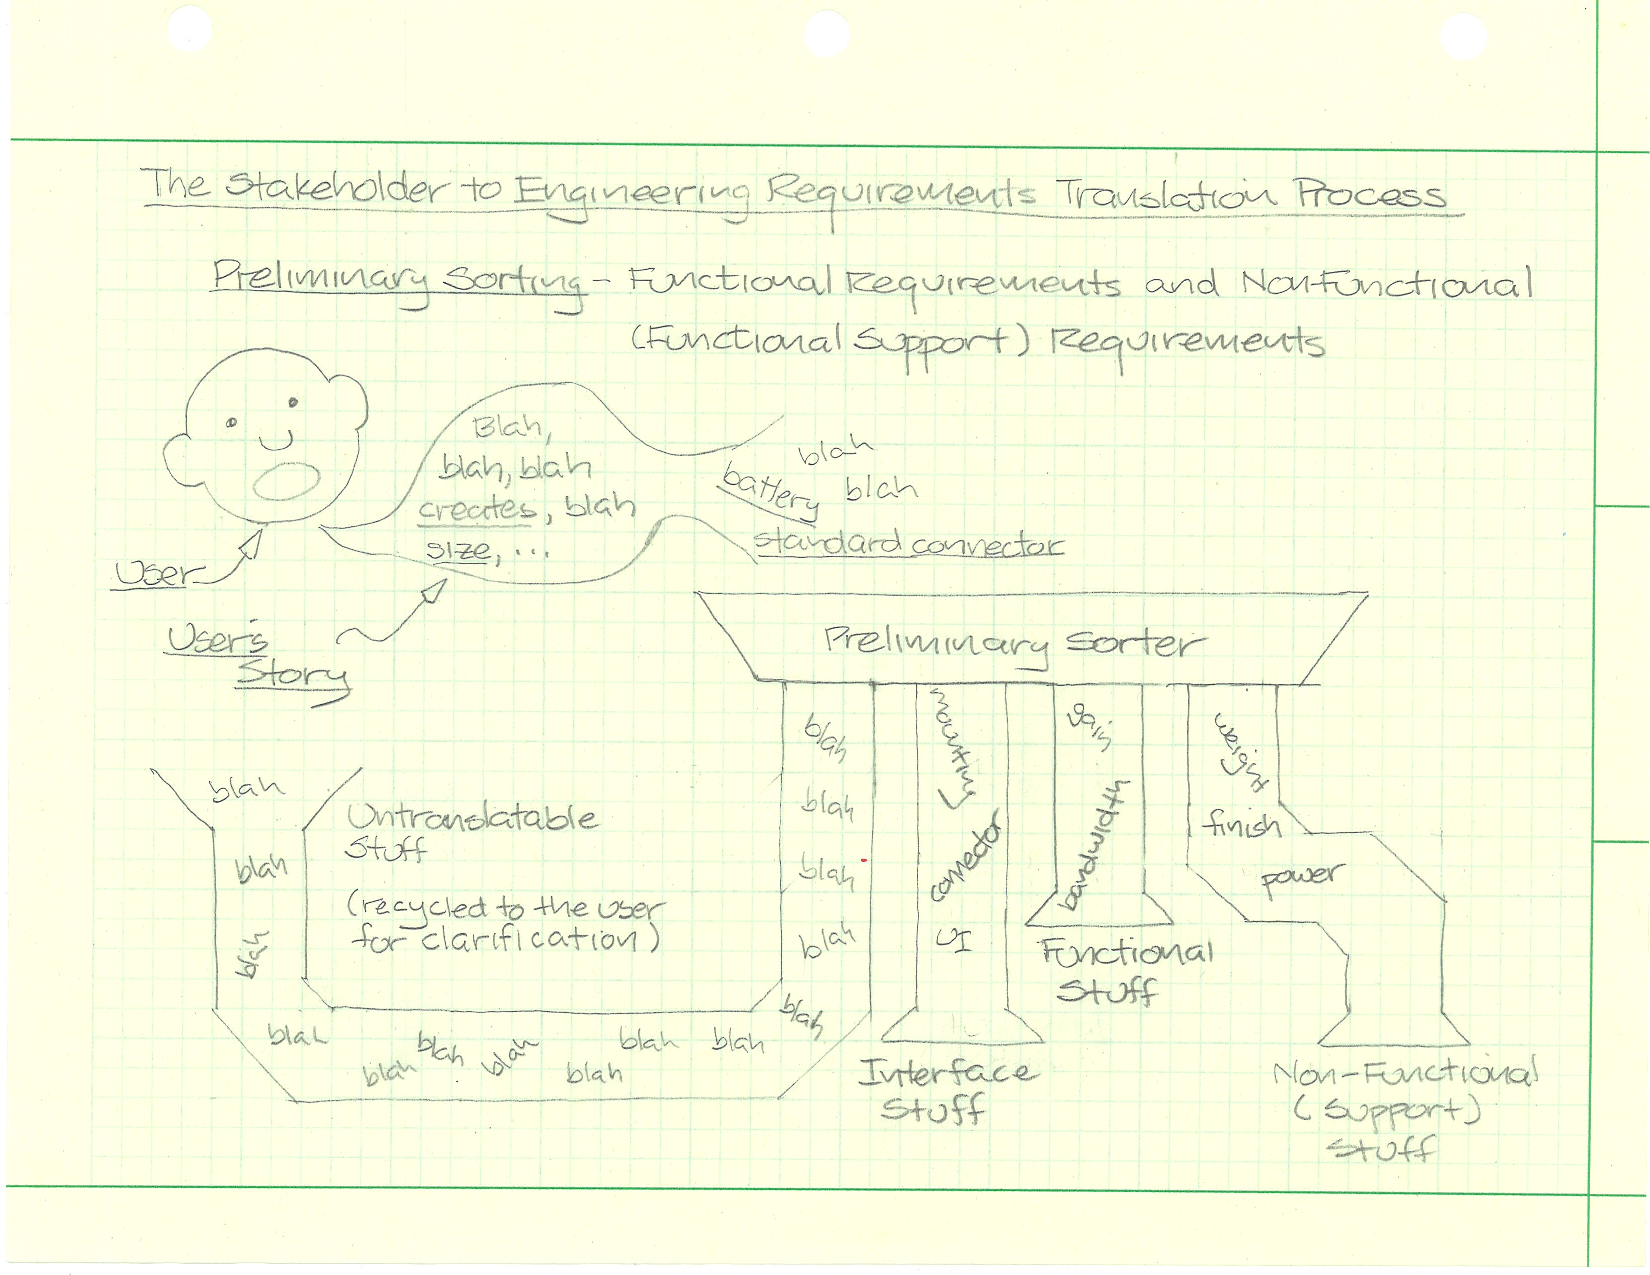
\includegraphics[angle=0,width=15cm]{PreliminarySorting.pdf}
%\caption{\label{fig:PreliminarySorting} A machine that sorts user stories into appropriate categories.}
%\end{figure}
%
%
%
%\begin{minipage}{\textwidth}
%	We will be sorting the requirements into four categories:
%	\begin{itemize}
%		\item Untranslatable Stuff
%		\item Interface Stuff
%		\item Functional Stuff
%		\item Non-Functional (Support) Stuff
%	\end{itemize}
%\end{minipage}
%
%\bigskip
%
%%These categories shown in the illustration are:
%%
%%\begin{enumerate}
%%\item \colorbox{Goldenrod}{Interface Constraints}
%%\item \colorbox{Lavender}{Method Constraints}
%%\item \colorbox{red}{Functional Requirements}
%%\item \colorbox{green}{Non-Functional Requirements (better called Functional Support Requirements)}
%%\item \colorbox{YellowOrange}{Options}
%%\item (Fluff)
%%\end{enumerate}
%%
%%The colors shown in the above list will be used to highlight pieces of the example stakeholder user stories that correspond to the categories.
%%\bigskip
%
%The categories themselves are intended to cover all aspects of the project in a systematic and an understandable fashion.  Properly chosen categories allow the designer working from this specification to verbally see the system (don't worry, we will also draw a few actual pictures of the system).  I'll explain the categories in the next sections.
%
%\paragraph*{Untranslatable Stuff}
%
%Let's face it we're human and our project stakeholders are human.  Being human we don't always communicate what is either meaningful or useful.  Sometimes, as engineers, when we hear or read a stakeholder statement it may seem vague or more like a wish.  Sometimes the statement may be incredibly obvious, but hard to translate into a measurable requirement.  When we encounter such statements it is up to us to approach the individual stakeholder and ask (politely) what on earth the statement means in terms of the project deliverables.
%\bigskip  
%
%Interacting with our stakeholders early in a project is a good thing.  We establish the lines of communication that we will most definitely need sometime in the project.
%\bigskip
%
%\paragraph*{Interface Stuff}
%
%We design and build things to perform some useful or interesting function.  Interesting things interact or interface with their environment to send information, provide motive power, receive and process information, receive power, fit into an existing slot, etc.  Interfaces make up the useful pieces of a system and are critical to the system.
%\bigskip
%
%The documentation for many complex systems includes a very useful document called an Interface Control Document, or ICD for short.  This document contains all the interface information for the system.  It is a very useful document and helps designers avoid a host of errors.  If such a document is available when the specification document is being written then it is simply referenced in the Applicable Documents Section of the specification.  For our purposes we will define the interface requirements as part of this specification document.
%\bigskip
%
%\paragraph*{Functional Stuff}
%
%The devices we make are intended to do something.  The something that they are supposed to do is defined as functional constraints (designer's hands tied) and functional requirements (designer is free to choose the method).
%\bigskip
%
%
%\paragraph*{Non-Functional (Support) Stuff}
%
%The engineered system is designed to produce certain things and interface in certain ways.  To accomplish its function the system needs a lot of support.  For example, a system is designed to process input data in a specific digital format and output the processed data in a specific digital format.  The format constitute interface constraints, but the connector for the digital formats constitute non-functional or functional support interface constraints.
%\bigskip
%
%The box that keeps the system from getting wet constitutes a non-functional or functional support requirement while the data processing requirements constitute a functional requirement.  Meeting non-functional requirements is as necessary to the system as meeting functional requirements.
%\bigskip
%
%Let's return to the example and start sorting the stakeholder user stories into the four categories.  The stories will be highlighted using four colors with the following meaning:
%\bigskip
%
%\end{slshape}
%
%\begin{enumerate}
%	\item \hilite{Cyan}{Untranslatable Stuff}
%	\item \hilite{Goldenrod}{Interface Stuff}
%	\item \hilite{Magenta}{Requirements Stuff}
%	\item \hilite{Apricot}{Non-Functional Stuff}
%\end{enumerate}
%
%\begin{slshape}
%\color{blue}
%Beginning with the Course Instructor's Pedagogical Requirements.  The marked version is:
%\end{slshape}
%\bigskip
%
%\begin{python}
%TheFile = open('CourseInstructorHandsOn.tex')
%
%lines = TheFile.readlines()
%
%markedLines = [0,3,6,9,12,15,18,21]
%
%hilite = ['Cyan','Cyan','Cyan','Magenta','Magenta','Magenta','Goldenrod','Magenta']
%
%for everyline in markedLines:
%
%    newstring = '\hilite{'+hilite[markedLines.index(everyline)]+'}{'+lines[everyline].rstrip('\n')+'}'
%
%    print(newstring+'\n'+'\\bigskip'+'\n')
%
%TheFile.close()
%\end{python}
%
%\begin{slshape}
%\color{blue}
%
%The Course Instructor's Pedagogical Requirements has one item classified as Interface Stuff dealing with the input impedance of the amplifier.  This item must be further sorted by the machine in Figure \ref{fig:InterfaceSorting}.  This machine determines if the item is a constraint or a requirement.
%
%\end{slshape}
%
%\begin{figure}[tb]
%\centering
%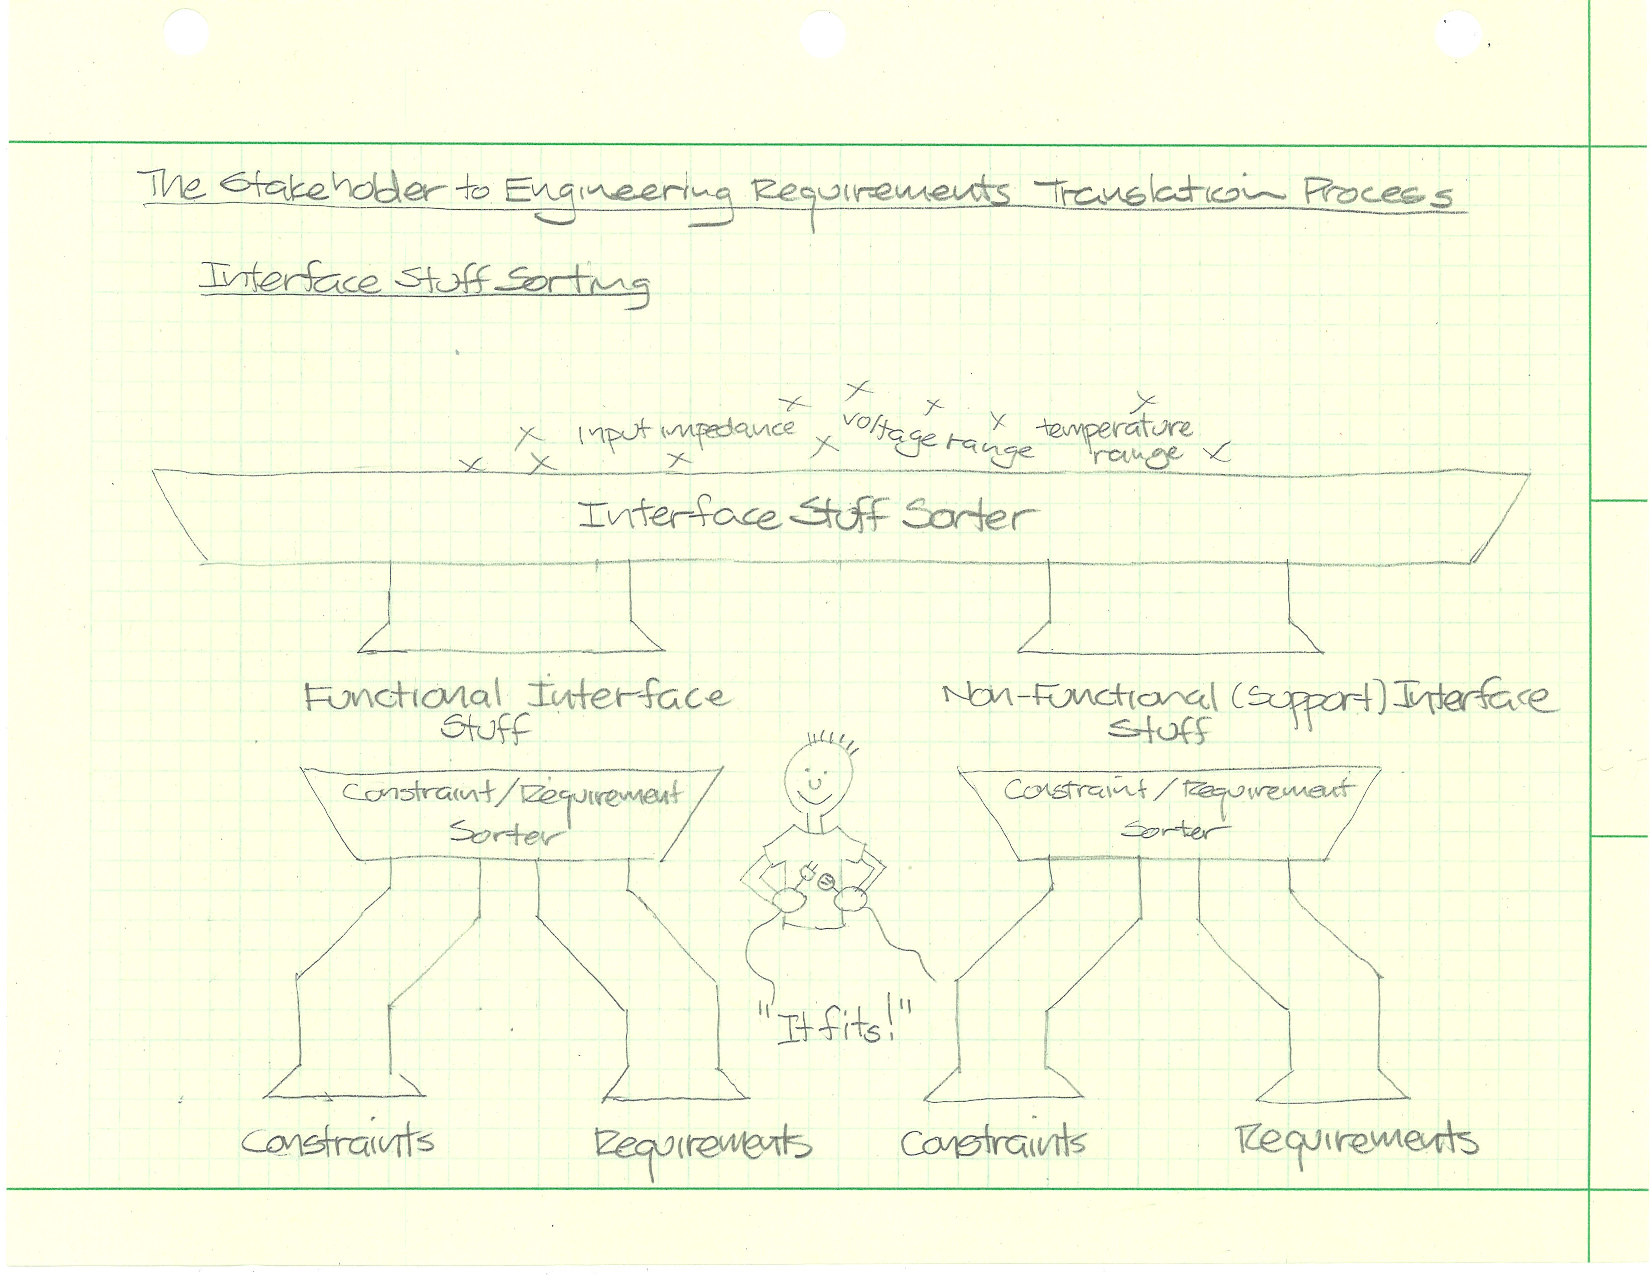
\includegraphics[angle=0,width=15cm]{InterfaceSorting.pdf}
%\caption{\label{fig:InterfaceSorting} A machine that sorts Interface Stuff into appropriate categories.}
%\end{figure}
%
%\begin{figure}[tb]
%\centering
%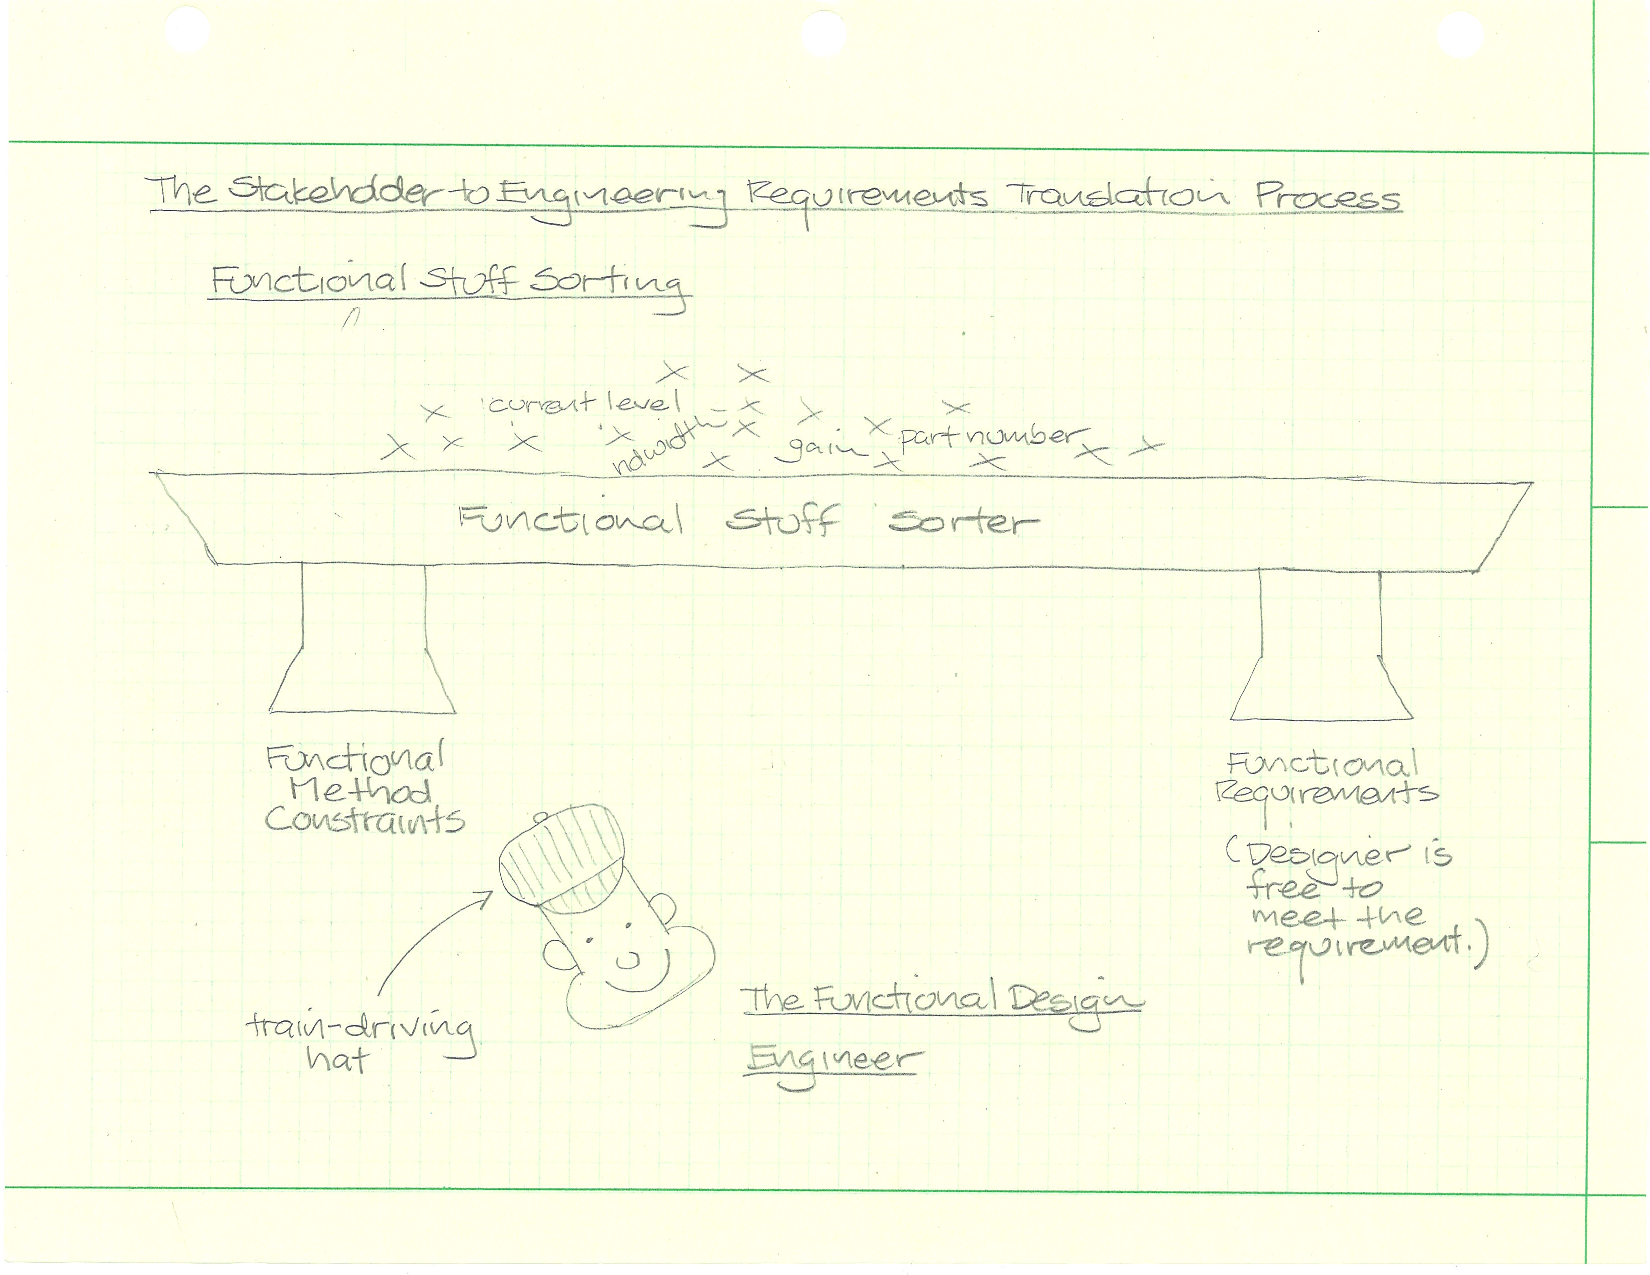
\includegraphics[angle=0,width=15cm]{FunctionalSorting.pdf}
%\caption{\label{fig:FunctionalSorting} A machine that sorts Functional Stuff into appropriate categories.}
%\end{figure} 
%
%\begin{figure}[tb]
%\centering
%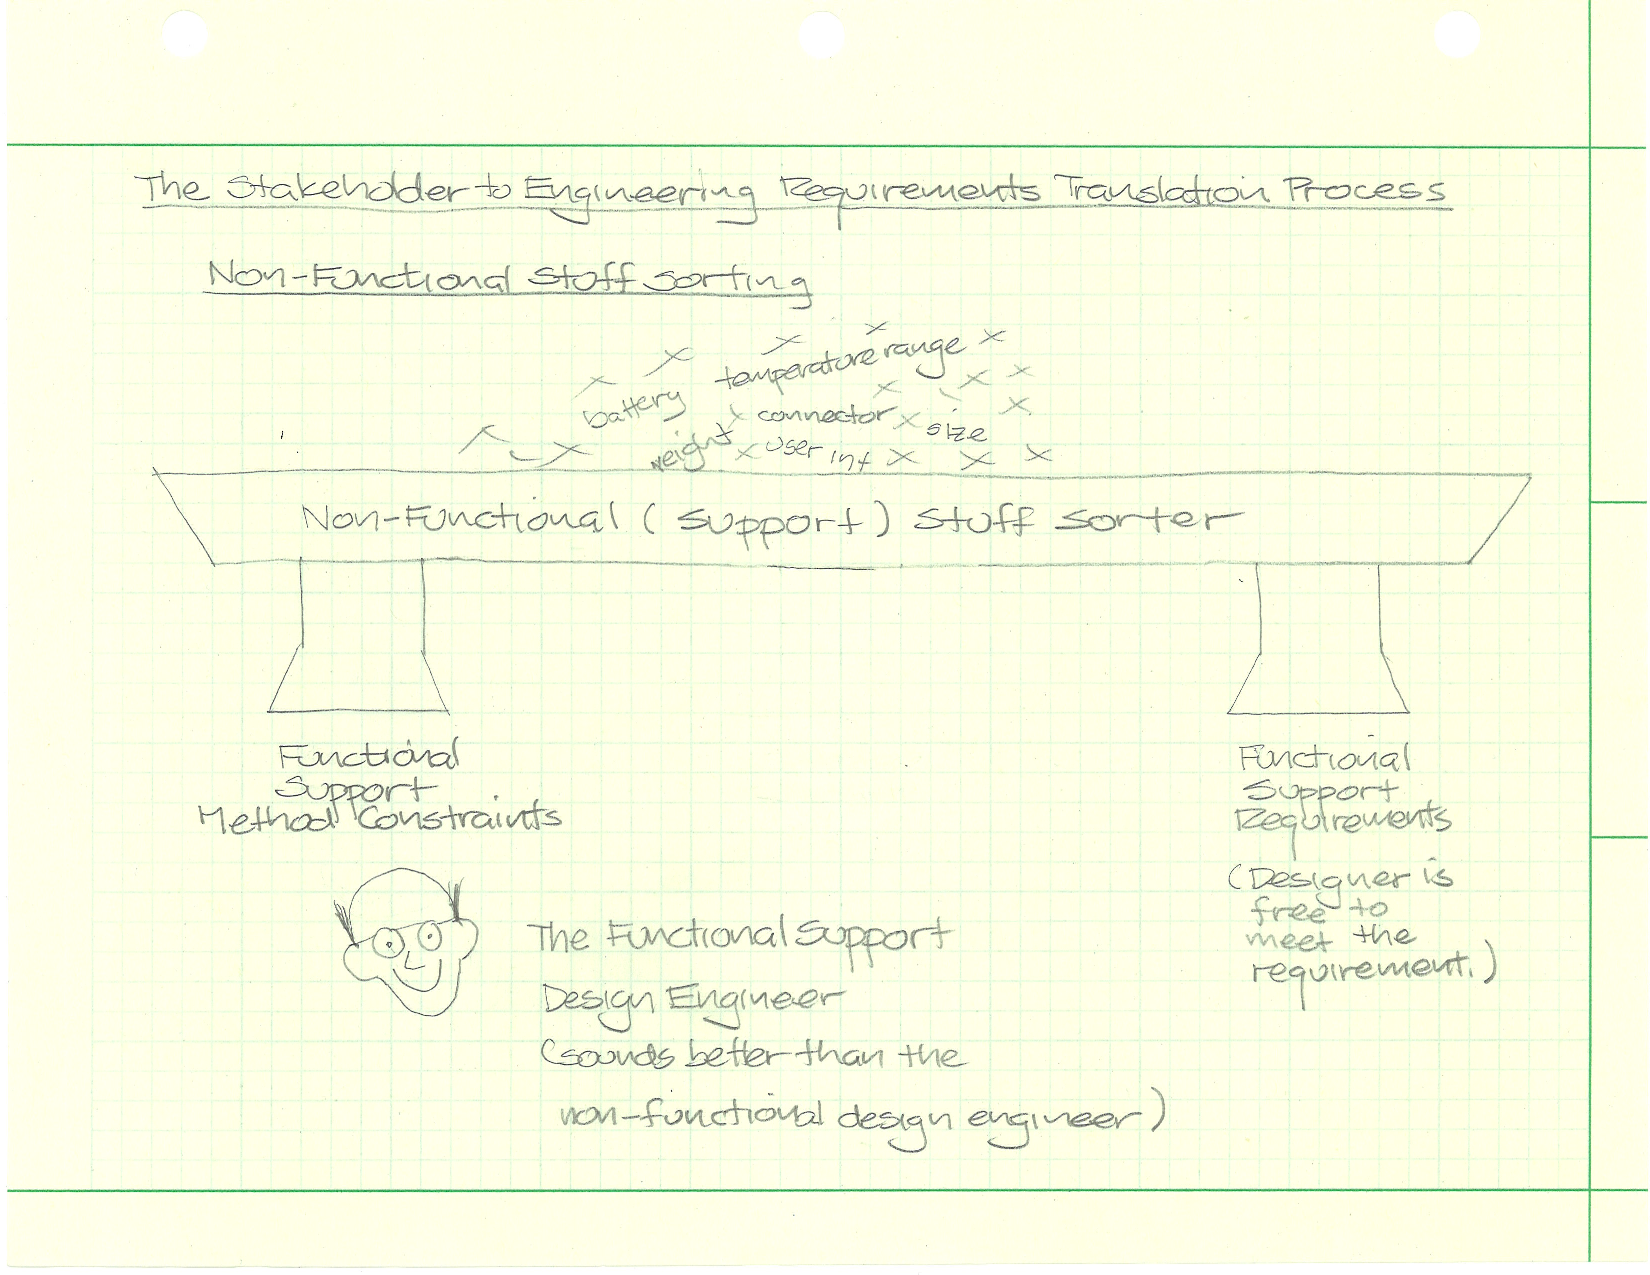
\includegraphics[angle=0,width=15cm]{NonFunctionalSorting.pdf}
%\caption{\label{fig:NonFunctionalSorting} A machine that sorts Non-Functional Stuff into appropriate categories.}
%\end{figure}
%

%
%
%
%
%
%\begin{slshape}
%
%
%
%
  %
%
%
%\paragraph*{Design Constraints}
%
%Constraining a system design amounts to designing part of the system rather than simply specifying it.  Constraint is necessary 
%for a variety of reasons including but not limited to: reuse of previously designed systems, existing capital equipment,  standard interfaces, and known 
%environmental conditions.
%\bigskip
	%
%As a rule designers hate constraints.  Designers are a vain bunch.  They see themselves as being the best person for the job and see 
%constraints as affronts to their competence.  You will save yourself needing to explain a constraint to an affronted designer by 
%explaining the constraint clearly in the specification (really clearly).
%\bigskip
%
%The sorting categories include two types of constraints:
%
%\begin{enumerate}
%\item Interface Constraints
%\item Method Constraints
%\end{enumerate}
%
%{\bf{\underline{Interface Constraints}}} exist because the functioning system must interface with something else.  One type of interface is a digital interface such as universal serial bus (USB) and the best way to express this interface constraint is to point to a Referenced Document and say `follow this'.  Analog interfaces are specified with such things as input impedance and voltage/current levels.  Typically simple human/machine interfaces can be specified in an engineering document but if you have to specify a complex human/machine interface there are standards for this type of problem also.  See, for example, the Apple user interface `requirements' are found here (\href{https://developer.apple.com/library/ios/documentation/UserExperience/Conceptual/MobileHIG/}{Apple User Experience Documentation}).  Again, why retype the wheel when you can just reference the wheel specification document.  Referenced documents really are your friend.
%\bigskip
%
%{\bf{\underline{Method Constraints}}} exist because a part of the system has been designed by the spec writer.  As an example a specific part number is stated in the specification and the designer is constrained to use this part to fulfill a requirement.  To reiterate \underline{explain your constraint} or be prepared to do a lot of explaining later.
%\bigskip
%
%\paragraph*{Requirements}
%
%I have divided the Requirements into Functional and Non-Functional Requirements.  In my view non-functional requirements are better understood as functional support requirements.
%\bigskip
%
 %
%
%
%
%
%\subsection*{Processing the Example User Stories}
%
%\end{slshape}
%
%
%\subsection*{Requirements and Constraints from the Course Instructor}
%
%\begin{itemize}
	%\item  {\textbf{The course instructor is the primary technical specifier of the controls lab power amplifier.  The device:}}
	%\begin{enumerate}
		%\item Must meet the pedagogical requirements of the course (ECE/MAE 5310) for which it is designed.\\[.5cm] \underline{User Story} \\
		%
%%\begin{python}
%%TheFile = open('CourseInstructorHandsOn.tex')
%%
%%for eachLine in TheFile:
    %%print(eachLine, end = '')
		%%
%%TheFile.close()
%%\end{python}
%\normalfont
%
	%\InputIfFileExists{CourseInstructorHandsOn.tex}
	%
%
%
		       %
%\bigskip
%
		  %
		%\item Must not present safety/shock hazards to any user.\\[.5cm] \underline{User Story} \\ 
		%
%\begin{python}
%TheFile = open('CourseInstructorSafety.tex')
%
%for eachLine in TheFile:
    %print(eachLine, end = '')
		%
%TheFile.close()
%\end{python}
		       %
		%
		%%As the course instructor, I need a safe module for the students to use.   Safety implies freedom from both electrical and mechanical hazzards.
		%%\bigskip
		%%
		%%The module must be free of sharp edges.
%%\bigskip
%
%% The structure below defines a text segment that I use again in the explanation.  I didn't want to have to change it in many places so it is defined as
%% a new command that I can typeset anywhere.
%
%%
	%%\global\def\voltageConstraint{The module must not present a dangerous shocking hazard to students.  In order to eliminate a potential dangerous shocking hazard the 
	%%power amplifier module supply voltages constrained to: $V_{+} \leq 18 \: \text{volts} \: \text{and} \: V_{-} \geq -18 \: \text{volts}$ or a total supply swing of $\leq 36$ Volts.}
	%
	%%\voltageConstraint
	%
%\bigskip
 	%
		%\item Must be robust so that student wiring errors do not damage the module.\\[.5cm] \underline{User Story}\\	
		%
%\begin{python}
%TheFile = open('CourseInstructorWiring.tex')
%
%for eachLine in TheFile:
    %print(eachLine, end = '')
		%
%TheFile.close()
%\end{python}
%\bigskip
	%
	%
		%\item Must be packaged to meet a specified envelope.\\[.5cm] \underline{User Story} \\
		%
%\begin{python}
%TheFile = open('CourseInstructorTSlot.tex')
%
%for eachLine in TheFile:
    %print(eachLine, end = '')
		%
%TheFile.close()
%\end{python}
%\bigskip
%
		%\item Must have a simple to understand interface that minimizes wiring mistakes.\\[.5cm] \underline{User Story}\\
		%
%\begin{python}
%TheFile = open('CourseInstructorBananaJacks.tex')
%
%for eachLine in TheFile:
    %print(eachLine, end = '')
		%
%TheFile.close()
%\end{python}
%\bigskip
		%
		%
	%\end{enumerate}
%
%\subsection*{Requirements and Constraints from the Laboratory Instructor}
%\subsection*{Requirements and Constraints from the Laboratory Student}
%\subsection*{Requirements and Constraints from the ECE Department}
%
%\subsubsection*{Finding Interface Constraints}
%
%Returning to the user stories in the example.  We can search them for constraints.
%
%%\item Must be robust so that student wiring errors do not damage the module.\\[.5cm] \underline{User Story}\\	
		%
%\begin{python}
%TheFile = open('CourseInstructorWiring.tex')
%
%for eachLine in TheFile:
    %eachLine = eachLine.replace('\colorbox{yellow}','')
    %"""eachLine = eachLine.replace('\colorbox{blue}','')"""
    %"""eachLine = eachLine.replace('\colorbox{red}','')"""
    %"""eachLine = eachLine.replace('\colorbox{green}','')"""
    %print(eachLine, end = '')
		%
%TheFile.close()
%\end{python}
%\bigskip
%
%\end{itemize}
%
%
%
	%
%\end{slshape}
%
%\subsection{Item Definition}
%
%\begin{slshape} \color{blue}
	%A more detailed description than SCOPE. Good idea to include an illustration. A listing of the major constituent parts or sub-assemblies 
	%is good here. A reference to the intended use and what the item is a part of goes here.
	%\bigskip
	%
	%You aren't limited to either one specific type of diagram or to a single diagram.  And since there is no perfect diagram you will
	%have to figure out what diagram or diagrams that will most clearly describe your system.  For example, an embedded system typically
	%has significant hardware and software requirements and hardware and software system diagrams are appropriate.
	%\bigskip
	%
	%Continuing with the power amplifier module example.
%\end{slshape}
%\bigskip
%
%\textbf{\underline{System Diagram}}   %(or appropriate system representation)
%\bigskip
%
%\begin{slshape} \color{blue}
	%All figures need a label centered on the page, one line below the figure. The label must 
	%follow this format (not the exact words):
%
	%\bigskip  
%
	%1. System data flow.
%\end{slshape}
%
%\subsection{Interface Definition}
%
%
%\begin{slshape} \color{blue}
	%All the "\,goes-intas and goes-outas." Further define the items 
	%covered in the System Diagram.
%\end{slshape}
%
%\begin{enumerate}[(a)]
	%\item Physical:
		%\begin{slshape} \color{blue}
			%Mounting, fluid interface, heat transfer if any, and so forth.  Using the controls lab power amplifier module as an example, the module has a size requirement, a mounting requirement, and a thermal interface with the environment requirement.  These are briefly described below.  Details are deferred at this point.
		%\end{slshape}
		%\subsubsection{Module Size}
		%
		%\subsubsection{Module Mounting}
		%
		%\subsubsection{Module Thermal Interface}
		%
		%The module shall interface with the lab environment through a passive heatsink.  Specific thermal requirements are found in paragraph %\ref{thermalManagement}.
		%\bigskip
		%
	%\item Electrical:
		%\begin{slshape} \color{blue}
			%Electrical connectors with pin diagrams as illustrations.	
		%\end{slshape}
		%
		%\subsubsection{Connector Requirements}
		%
		%\subsubsection{Electrical Interface Requirements}
		%
		%\paragraph{Input Voltage Range}
		%
		%\subparagraph{} 
		%The controls lab power amplifier module shall amplify input voltage signals of $\pm 10$ volts within the gain specifications of paragraph \ref{gainSpec}.
		%
		%\subparagraph{} 
		%The controls lab power amplifier shall withstand, without damage, input voltages up the supply rails of the amplifier.
		%
		%\paragraph{Output Voltage Range}
		%
		%\subparagraph{}
		%The controls lab power amplifier module shall produce output voltages per the requirements of paragraph \ref{gainSpec}.
		%
		%\paragraph{Input Impedance}
		%
		%The controls lab power amplifier module shall have an input resistance of no less than $10K\Omega$.
		%
		%\paragraph{Output Impedance}
		%
		%The controls lab power amplifier module shall appear a resistive load as a ideal voltage source in series with a resistance of $\le 0.01\Omega$.
		%
		%
		%
	%\item Functional or Informational
		%\begin{slshape} \color{blue}
			%What data goes in and out, what does what to what. Data bus 
			%definition (i.e. MIL-STD-1553 or RS-232, etc.) would go here if needed.
		%\end{slshape}
	%
%\end{enumerate}
%
%\begin{slshape} \color{blue}
	%The following sections are the focal point of the REQUIREMENTS section. The outline may be 
	%expanded as needed to provide the necessary depth of explanation. Remember to state requirements
	%in the imperative, "shall".		
%\end{slshape}
%
%
%%\subsection{Design Constraints}
%%
%%
%%\begin{slshape} \color{blue}
	%%Constraining a system design amounts to designing part of the system rather than simply specifying it.  Constraint is necessary 
	%%for a variety of reasons including but not limited to: reuse of previously designed systems, existing capital equipment,  and known 
	%%environmental conditions.
	%%\bigskip
	%%
	%%As a rule designers hate constraints.  Designers are a vain bunch.  They see themselves as being the best person for the job and see 
	%%constraints as affronts to their competence.  You will save yourself needing to explain a constraint to an affronted designer by 
	%%explaining the constraint clearly in the specification (really clearly).
	%%\bigskip
	%%
	%%Continuing with the power amplifier module as an example, we will try to ferret out design constraints from the stakeholder's user stories.
	%%\bigskip
	%%
	%%Use of the word `constraint' in a user's story is a dead give away, but we don't always find the exact word and we will have to work a little harder
	%%to separate constraints from requirements.
	%%\bigskip
	%%
	%%From the course instructor's User's Story we find the word \underline{constrained} used in the following:
	%%
	%%\begin{quote}
	 %%As a course instructor I need equipment in the control systems lab that provides students with a useful hands-on experience.
\bigskip
  
In order to be useful the lab equipment used must not be mysterious (or overly 'black box').
\bigskip
  
Students need to see the inputs and outputs of the system and understand that they can replicate similar systems in their careers.
\bigskip
		
The power amplifier module must be constructed of a technology that is familiar to both mechanical and electrical/computer engineering students at a late-junior year level.  In order to meet this familiarity requirement the design is constrained to use a power operational amplifier.
\bigskip
		
The power amplifier needs to be a unity voltage gain non-inverting buffer. 
\bigskip

The power amplifier must provide a minimum continuous output current of 8 amps.
\bigskip

The input impedance of the power amplifier must be greater than or equal to 10 kilohms.
\bigskip
		
The largest time constant of the power amplifier must be less than 0.001 seconds.
\bigskip
	%%\end{quote}
	%%
	%%We can now safely write our first design constraint.
	%%
%%\end{slshape}
%
%\subsubsection{Amplifying Element Constraint}
%
%The controls lab power amplifier module shall use a commercially available power operational amplifier as it amplifying element.  This constraint is placed on the module design
%because of mechanical and electrical/computer engineering student familiarity with operational amplifiers.
%\bigskip
%
%\begin{slshape} \color{blue}
%Continuing with the course instructor's user story, we look for other instances of words similar to constraint.
%\bigskip  
%
%It didn't take long to find the next one.
%
%\begin{quote}
	%As the course instructor, I need a safe module for the students to use.   Safety implies freedom from both electrical and mechanical hazards.
\bigskip
		
The module must be free of sharp edges.
\bigskip
		
The module must not present a dangerous shocking hazard to students.
\bigskip

In order to eliminate a potential dangerous shocking hazard the power amplifier module supply voltages are constrained to: $V_{+} \leq 18 \: \text{volts} \: \text{and} \: V_{-} \geq -18 \: \text{volts}$ or a total supply swing of $\leq 36$ Volts.
\bigskip
%\end{quote}
%
%This constraint is troublesome.  While the course instructor really doesn't want to shock students (a rare instructor indeed), the designer of this module has little control over the power supply voltages.  The responsibility for these voltages is likely fixed by available equipment.  The course instructor would have been better off stating that, due to available lab equipment, the power supply voltages are limited to a maximum of $\pm V$.  An even better constraint would set a range of acceptable voltages such as 12 to 18 volts. Let's write this constraint in that way.
%\bigskip 
%
%\end{slshape}
%
%\subsubsection{Power Supply Voltage Constraint}
%
%The control power operational amplifiers shall operate on power supplies with output voltages symmetric about a ground reference voltages $\lvert {V_{+}} \rvert = \lvert {V_{-}} \rvert = V$  with $V$ in the range of $10 \:\text{volts} \le V \le 18 \: \text{volts}$.  The power supply voltages of the power amplifier module are constrained to these value due to the availability of laboratory power supplies that operate in this range.
%\bigskip
%
%\begin{slshape}
%\color{blue}
%
%Continuing the search for constraints in the stakeholder's user stories.  The next course instructor comment mentions:
%\end{slshape}
%
\subsection{Item Definition} 
The Backyard Splash Pad is comprised of four main components: a device controller, a user interface, a mechanical system, and an object-tracking system. 
The device controller receives input from the user interface and uses it to control the mechanical system.
The user interface presents information about the system to the user and accepts input from the user.
The mechanical system controls the flow of water. 
The object-tracking system detects objects near the Splash Pad and reports information to the controller. 
See Figure \ref{fig:functional_diagram}.

\subsubsection{Functional Diagram}

\begin{figure}[h]
\begin{centering}
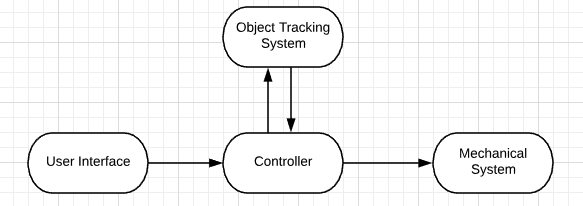
\includegraphics{Functional_Diagram.png}
\caption{\label{fig:functional_diagram}Functional Diagram.}
\end{centering}
\end{figure}

\subsection{Functional Requirements}

\subsubsection{Device Controller Functional Requirements}

\subsubsection{User Interface Functional Requirements}

\subsubsection{Mechanical System Functional Requirements}

\subsubsection{Object Tracking System Functional Requirements}

\subsection{Support Requirements}

\subsubsection{Device Controller Support Requirements}

\subsubsection{User Interface Support Requirements}

\subsubsection{Mechanical System Support Requirements}

\subsubsection{Object Tracking System Support Requirements}



%\begin{quote}
	%\input{CourseInstructorMounting}
%\end{quote}
%
%Now is good time to discuss the difference between design constraints and requirements.  Why don't we treat the rail mounting constraint as a requirement?  We could and often we would by simply specifying an exact mounting structure for the power amplifier with no explanation of why it has to be the size and shape that it must be.  However, the rail mounting system is an external standard that we must follow and my experience tells me that informing the designer of the reason for this constraint keeps the designer happier.  And happier designers mean happier spec writers!
%\bigskip
%
%At this point we can simply state the fundamental constraint and leave the actual mounting envelope sizes to another place in the document (probably the Interface section) or we can state the complete requirement here.  I choose to put it here and back reference it in the requirements simply because it is a constraint and splitting the needed data into two places could lead to interpretation errors.  The rail mounting constraint follows.
%\bigskip
	%
%\end{slshape}
%
%\subsubsection{Rail Mounting Constraint}
%
%
%\paragraph{} 
%
%The controls lab power amplifier module shall be packaged in a structure that mounts to the 1 inch t-slot railing used in the lab via two $1/4$ inch holes in the bottom of the structure that are separated by no more than two inches.
%
%\paragraph{} 
%
%The module package dimension along the rail shall be no more six inches.
%
%\begin{slshape}
%\color{blue}
%
%We can now look for other constraints in the stakeholders' user stories.  The last course instructor user story uses indefinite words such as 'need', `can', and `recommended'.  These words imply latitude in implementation and as such will be expanded in the appropriate requirements section.
%\bigskip
%
%The lab instructor user stories yield needs no specific constraints.  Remember even a specific requirement is not a constraint if no specific method is expressed.
%\bigskip
%
%The lab student user stories also have needs but without expressing specific methods.  No constraints here.
%\bigskip
%
%The USU ECE Department user stories have flirtations with constraints but never quite get there with phases such as `must be a simple' and 'should cost less'.  While the Department may be sincere about these requirements they are not constraining the designer to a specific method to achieve them (they aren't even really requiring them).
%\bigskip
%
%\end{slshape}
%
%\subsection{Functional Requirements}
%
%\begin{slshape} \color{blue}
	%A quantitative statement of how the item does what is
	%does. For a thruster it would be thrust, specifc impulse and stability. For a power supply
	%it would be current, voltage, and efficiency. Times like rise times, fall times, and
	%transients are defned here. Leakage (uid or current) is usually defined here.
	%Compatibility with fluids is often defined here. It is a good idea to start with a previous
	%spec for a similar item to get some ideas for all that may need to be in this section.
	%Curves, truth tables, and functions are often better than words for these requirements.	
%\end{slshape}
%
%\subsubsection{Amplifier Functional Characteristics}
%
%\paragraph{Voltage Gain Requirement}\label{gainSpec}
%
%The controls lab power amplifier shall have the following steady state transfer function (voltage gain):
%\bigskip
%
%\begin{math}
	%\dfrac{V_{out}}{V_{in}} = 1.0 \pm 1\%
%\end{math}
%
%\paragraph{Output Current Requirements}
%
%The controls lab power amp shall have a maximum steady state output current of no less than 8 amps.
%
%\paragraph{Bandwidth}
%
%The controls lab power amplifier shall have a half power bandwidth of no less than 100 Hz.
%
%
%
%\subsection{Non-Functional Requirements}
%
%\begin{slshape} \color{blue}
%
%What follows is a really long (and yet strangely incomplete) list of potential non-functional requirements.  You will likely have noticed that the functional requirements for the controls lab power amplifier is a pretty short list.  Simple signals in and out and a frequency response requirement.  We should be able to stop this madness now and build the thing.  Sadly, we can't stop yet.
%\bigskip
%
%The device functions described in the section above don't and can't stand alone.  These functions require a lot of support from the environment.  To use a common example, the functions of a cell phone are simply dreams without the battery,  The functions of that same phone are useable only because of an effectively designed package.  Your cell phone is useful over a range of temperatures (a much smaller range than you are likely aware of (\href{https://support.apple.com/en-us/HT201678}{iPhone Temperature Ranges})) because the designers made it useful over the range of temperatures that were specified.  In short, function is meaningless without a non-functional framework or, in other words, a functional support framework.
%\bigskip
%
%Our example is no different.  The amplifier must be supplied with power.  It must be able to operate over a range of temperatures and dissipate heat so as to keep the amplifying element safe.  It must be packaged to make it possible for us to actually use it.  We specify those requirements in this section and include the list of a bunch of others that may or may not apply to our specific project.
%\bigskip
%
%Returning to the user stories we look for the requirements that the users have provided that can be classified as non-functional requirements.  The first one we encounter deals with the electrical wiring and it seems reasonable then to group electrical support (non-functional) issues into their own section.  The course instructor requires:
%\bigskip
%
%\WiringErrors
%\bigskip
%
%Looking for more electrical requirements we find:
%\bigskip
%
%\OverCurrent
%\bigskip
%
%and the lab instructor suggests:
%\bigskip
%
%\BananaJacks
%\bigskip
%
%The lab instructor requires:
%\bigskip
%
%\UserWiringInterface
%
%
  %
%
%Lets' divide this section into the following subsections:
%
%\begin{itemize}
	%\item Electrical Requirements
	%\begin{itemize}
		%\item Power Protection Requirements
		%\item Connector Requirements
	%\end{itemize}
	%\item{Environmental Requirements}
	%\begin{itemize}
		%\item Operating Temperatures
		%\item Power Dissipation
	%\end{itemize}
	%\item Physical Characteristics
	%\begin{itemize}
		%\item Packaging
		%\begin{itemize}
			%\item Package Envelope
			%\item Rail Mount
		%\end{itemize}
	%\end{itemize}
%\end{itemize}
%
%Starting with the electrical requirements we continue our example.
%\end{slshape}
%
%\subsubsection{Electrical Requirements}
%
%\begin{slshape} \color{blue}
%
%\end{slshape}
%
%\paragraph{Power Protection Requirements} 
%
%\begin{slshape} \color{blue}
%
%\end{slshape}
%
%\paragraph{Connector Requirements}
%
%\subsubsection{Environmental Requirements}
%
%\begin{slshape} \color{blue}
%{\underline{Environments}}
	%
	%\bigskip
%
	%This section is for anything and everything that is external 
	%to the item that it must withstand. Customers may impose these with an 
	%Environmental Requirements Document. Margins should be added beyond 
	%hard environmental limits that would damage the item. NOTE: MOST OF THIS 
	%IS THE SAME FOR ALL SUBSYSTEMS AND WILL THEREFORE BE WRITTEN INTO THE 
	%SYSTEMS SPEC.
	%
	%\bigskip
%
	%{\underline{Natural Environments}}
	%
	%\bigskip
%
	%Anything that is relevant to the item that can occur in the 
	%natural world, either prior to use or during use. Some words like 
	%"The item shall meet the requirements of this specification 
	%during and after exposure to any combination of any of the following 
	%natural environments. The item may be packaged to precluded exposure to 
	%any environments that would control the design." Typical environments 
	%include (but are not limited to):
	%
	%\bigskip
%
	%External Pressure, remember barometric and transportation in 
	%unpressurized aircraft. Also rate of pressure change.
	%
	%\bigskip
%
	%Temperature including both operating and non-operating. Some 
	%special temperatures may include freezing points of consumables like 
	%fuels.
	%
	%\bigskip
%
	%Salt spray or other corrosives, lightning, and magnetic fields.
	%
	%\bigskip
%
	%{\underline{Induced Environments}}
	%
	%\bigskip
%
	%Anything that is relevant to the item that is caused by 
	%human-made objects, either prior to use or during use. Some words like 
	%\textsl{"\,The item shall meet the requirements of this specification 
	%during and after exposure to any logical combination of the following 
	%natural environments." } Typical environments include (but not limited 
	%to):
	%
	%\bigskip
%
	%Mechanical shock, including transportation and use. Amplitude and 
	%number of shocks can be defined in either the time domain or frequency 
	%domain.
	%
	%\bigskip
%
%
	%Vibration, including transportation and use. Amplitude as a 
	%function of frequency is the usual format. Duration is a key part of 
	%this requirement.
	%
	%\bigskip
%
	%Acoustic input
	%
	%\bigskip
%
	%Load factors and acceleration
	%
	%\bigskip
%
	%Space Environment including Radiation, Atomic Oxygen. Radiation is 
	%a specialty area that includes cosmic radiation, charged particles in 
	%the solar wind and Van Allen radiation in some orbits. Atomic oxygen is 
	%of concern for polymers and nonmetallic materials exposed on the front 
	%of the spacecraft (with reference to the velocity vector) in orbits 
	%under 500 km altitude.
	%
	%\bigskip
%
	%Spacecraft develop charges when moving through the earth's 
	%magnetic field in the continuous presence of charged particles. 
	%Increased solar wind can alter the magnitude of the charge. Design 
	%features may be needed to diminish charge separation within a 
	%spacecraft, make electronics less vulnerable to accumulated charge, and 
	%in the case of rendezvous and docking allow for harmless dissipation of 
	%accumulated charges between spacecraft.
	%
	%\bigskip
%
	%External Pressure, remember barometric and transportation in 
	%unpressurized aircraft. Also rate of pressure change.
	%
	%\bigskip
%
	%Temperature during operation. Also thermal cycling and 
	%thermal/vacuum. 
	%
	%\bigskip
%
%
	%Cleanliness: Cleanliness is, of course, next to Godliness, and that is 
	%even more true that you realize for spaceflight hardware. This section 
	%usually controls particulate and fiber cleanliness with tables of 
	%allowable count per range of particle size. Surface cleanliness is also 
	%controlled. The use and certification of cleanrooms is controlled in 
	%this section. Special issues such as propellant contacting surfaces, 
	%flushing fluid components, and electronic cleanliness are controlled 
	%here. NOTE: MOST OF THIS IS THE SAME FOR ALL SUBSYSTEMS AND WILL 
	%THEREFORE BE WRITTEN INTO THE SYSTEMS SPEC.
	%
	%\bigskip
%
	%Electromagnetic interference (EMI):  The unit shall met the EMI 
	%requirements for class xxx equipment as specified in 
	%MIL-STD-461, except for yyy limits shall be modified as shown 
	%in Figure zzz.  This is typical language, and MIL-STD-461 
	%is still commonly used. Emissions, refer to EMI that originates in the 
	%unit that can negatively affect other things. Susceptibility refers to 
	%unexpected negative effects on the unit that are caused by emissions 
	%from some other source. Self-susceptibility is a special case when 
	%electrical noise created by the unit triggers and unexpected effect 
	%within the unit. EMI can be "conducted" along power or 
	%signal wires or "radiated." The MIL-STD-461 limits have coded names 
	%like:
	%
	%\bigskip
%
	%CS01 = conducted susceptibility in the first frequency range, RE02 = 
	%radiated emissions in the second frequency range.
	%
	%\bigskip
%
	%Magnetic fields are another category controlled by the MIL-STD. Testing 
	%methods are usually defined by an associated methods document, 
	%MIL-STD-462. Other parts or sub-paragraphs in this section deal with 
	%electrical bonding (specified minimum resistance) between different 
	%subassemblies, EMI gasket and screen materials, grounding, lightning 
	%transients, and shielding.
%\end{slshape}
%
%\subsubsection{Physical Characteristics}
%
%\begin{slshape} \color{blue}
%{\underline{Physical Characteristics}}
	%
	%\bigskip
	%This is the place for the envelope drawing that shows size 
	%and general configuration. Sensitive areas, keep-out zones, and dynamic 
	%envelopes should be defined here. The mass, mass moment of inertia, 
	%center of mass, and natural frequency requirements can be defined here. 
	%Any unusual orientation requirements (e.g. "\,this side up") can be 
	%defined here. Location requirements for electrical connectors or 
	%tube-fitting interfaces should be defined. Visual indicators or 
	%inspection zones or tool access zones should be identified.
	%
	%\bigskip
%\end{slshape}		